\chapter{Critiques and Nuances of the Compression Phase}

\section{The Deterministic Mapping Problem}

The Information Bottleneck (IB) theory of deep learning, particularly the influential claim that training a neural network naturally decomposes into a brief ``fitting'' phase followed by a prolonged ``compression'' phase, has sparked intense debate. In the standard narrative, as learning progresses, the network sheds irrelevant information about the input $X$ while preserving information relevant to the target $Y$. This dynamic is elegantly visualized as a trajectory in the information plane, tracing the mutual information $I(X; T)$ against $I(T; Y)$, where $T$ represents the hidden layer activations. In this view, learning is fundamentally a process of extracting a minimal sufficient statistic.

However, a fundamental critique arises when we scrutinize the nature of modern neural networks. The original experiments demonstrating the compression phase heavily relied on specific architectural choices---notably, the use of saturating activation functions like $\tanh$, and the estimation of mutual information via discretization (binning) of the hidden activations. When researchers attempted to replicate these findings using the ubiquitous Rectified Linear Unit (ReLU) and non-binned estimators, the crisp picture of compression began to blur. Networks constructed with ReLU activations did not seem to exhibit a measurable decrease in $I(X; T)$ during the later epochs of training, casting doubt on the universality of the compression phase.

The most profound theoretical critique centers on the definition of mutual information itself in deterministic systems. A standard feedforward neural network computes a deterministic function of its input. If the input $X$ is a continuous random variable and the mapping from $X$ to $T$ is deterministic and sufficiently well-behaved, the mutual information $I(X; T)$ is strictly infinite. This mathematical reality poses a severe challenge to the empirical observation of a changing $I(X; T)$. If the true mutual information is vacuous or infinite, what exactly were the original IB experiments measuring?

This chapter dissects these critiques. We begin by formalizing the pathologies of mutual information in deterministic networks, showing that what appears to be information compression may in fact be an artifact of binning or the saturation of activation functions. We then explore alternative interpretations, such as geometric clustering, which suggest that while the \emph{informational} volume might not decrease in a well-defined Shannon sense, the \emph{geometric} volume of the representations certainly does. By resolving these nuances, we aim to preserve the powerful intuition of the Information Bottleneck while grounding it in mathematically rigorous footing that applies to the networks used in practice today.

\section{Mathematical Pathologies of Mutual Information}

\subsection{Infinite Mutual Information in Continuous Deterministic Systems}

To understand the critique of the compression phase, we must formally evaluate $I(X; T)$ when $T = f_\theta(X)$ is a deterministic transformation parameterized by $\theta$.

\begin{theorem}[Infinite Mutual Information in Deterministic Networks]
\label{thm:infinite_mi}
Let $X \in \mathbb{R}^d$ be a continuous random variable with a strictly positive probability density function on its support. Let $f_\theta: \mathbb{R}^d \to \mathbb{R}^m$ be a deterministic, piecewise continuously differentiable function representing a neural network layer, and let $T = f_\theta(X)$. If $f_\theta$ is injective on any open set of the support of $X$, then the mutual information $I(X; T)$ is infinite.
\end{theorem}

\begin{proof}
Recall the definition of mutual information for continuous random variables:
\[
I(X; T) = h(T) - h(T | X)
\]
Since $T$ is completely determined by $X$, the conditional distribution $p(t | x)$ is a Dirac delta function $\delta(t - f_\theta(x))$. The differential entropy of a Dirac delta function is negatively infinite:
\[
h(T | X) = \int p(x) \int \delta(t - f_\theta(x)) \log \frac{1}{\delta(t - f_\theta(x))} \, dt \, dx \to -\infty
\]
Assuming the marginal differential entropy $h(T)$ is finite (which holds if $T$ has a bounded density), we are subtracting a negatively infinite quantity, yielding $I(X; T) = \infty$.

Alternatively, evaluating the Kullback-Leibler divergence between the joint and the product of marginals:
\[
I(X; T) = D_{\text{KL}}(P(X, T) \parallel P(X)P(T)) = \int \int p(x, t) \log \frac{p(x, t)}{p(x)p(t)} \, dx \, dt
\]
The joint distribution $p(x, t)$ is singular with respect to the product distribution $p(x)p(t)$. Specifically, all the probability mass of $p(x,t)$ lies on the lower-dimensional manifold $t = f_\theta(x)$, which has measure zero in the product space $\mathbb{R}^d \times \mathbb{R}^m$. Therefore, the Radon-Nikodym derivative does not exist, and the divergence evaluates to $+\infty$.
\end{proof}

This theorem highlights a critical flaw: for deterministic networks without injected noise, the quantity $I(X; T)$ is a mathematical constant (infinity) and cannot dynamically change during training. The observed ``compression'' must therefore stem from the estimation procedure rather than the true Shannon mutual information.

\begin{figure}[htbp]
\centering
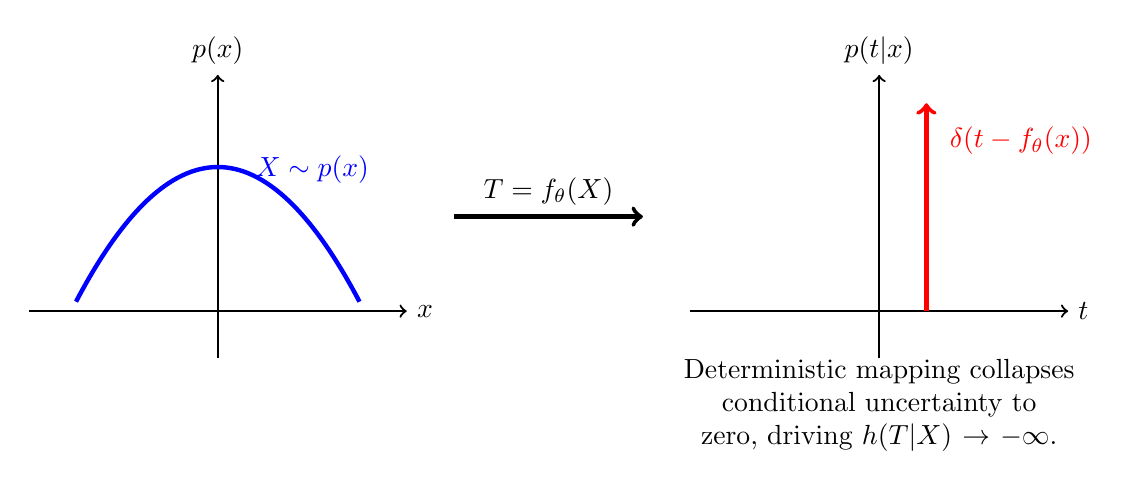
\begin{tikzpicture}[scale=1.2]
    % Axes for X
    \draw[->, thick] (-2,0) -- (2,0) node[right] {$x$};
    \draw[->, thick] (0,-0.5) -- (0,2.5) node[above] {$p(x)$};
    % PDF of X
    \draw[ultra thick, blue] (-1.5,0.1) .. controls (-0.5,2) and (0.5,2) .. (1.5,0.1);
    \node[blue] at (1,1.5) {$X \sim p(x)$};

    % Arrow for deterministic function
    \draw[->, ultra thick] (2.5, 1) -- (4.5, 1) node[midway, above] {$T = f_\theta(X)$};

    % Axes for T
    \draw[->, thick] (5,0) -- (9,0) node[right] {$t$};
    \draw[->, thick] (7,-0.5) -- (7,2.5) node[above] {$p(t|x)$};
    
    % PDF of T - Dirac delta
    \draw[ultra thick, red, ->] (7.5,0) -- (7.5,2.2);
    \node[red] at (8.5,1.8) {$\delta(t - f_\theta(x))$};
    
    \node[align=center, text width=5cm] at (7, -1) {Deterministic mapping collapses   conditional uncertainty to zero,   driving $h(T|X) \to -\infty$.};
\end{tikzpicture}
\caption{In a deterministic neural network, the mapping from the input $X$ to the representation $T$ is absolute. The conditional probability $p(t|x)$ is a Dirac delta, making the mutual information strictly infinite.}
\label{fig:deterministic_mapping}
\end{figure}

\subsection{The Illusion of Compression via Binning}

If the true mutual information is infinite, why did early empirical studies observe a distinct compression phase? The answer lies in the estimation method. To compute $I(X; T)$ computationally, early works partitioned the continuous range of $T$ into discrete bins, essentially measuring the information of a quantized variable, $\hat{T}$.

\begin{theorem}[Binned Mutual Information]
Let the range of $T \in \mathbb{R}^m$ be partitioned into uniform hypercubical bins of side length $\Delta$. Let $\hat{T} = [T]_\Delta$ be the discrete binned variable. As $\Delta \to 0$, the mutual information of the binned representation satisfies:
\[
I(X; \hat{T}) \approx H(\hat{T}) \approx h(T) - m \log \Delta
\]
assuming $T$ has a continuous and bounded probability density function.
\end{theorem}

\begin{proof}
Because $T$ is a deterministic function of $X$, the binned variable $\hat{T}$ is also entirely determined by $X$. Therefore, the discrete conditional entropy $H(\hat{T} | X) = 0$. 
It follows directly that $I(X; \hat{T}) = H(\hat{T}) - H(\hat{T} | X) = H(\hat{T})$.
From standard information theory, the discrete entropy of a finely quantized continuous variable is related to its differential entropy by:
\[
H(\hat{T}) = h(T) - \log(\Delta^m) + \mathcal{O}(\Delta) = h(T) - m \log \Delta + \mathcal{O}(\Delta)
\]
Thus, for sufficiently small $\Delta$, $I(X; \hat{T}) \approx h(T) - m \log \Delta$.
\end{proof}

This result is revealing. The measured mutual information $I(X; \hat{T})$ is essentially tracking the differential entropy $h(T)$ of the hidden representations, shifted by a constant that depends arbitrarily on the bin size $\Delta$. The perceived ``compression of information from $X$'' is actually just a reduction in the differential entropy of $T$.

\subsection{Numerical Example: Saturation and Differential Entropy}

Why would the differential entropy $h(T)$ decrease during training? Consider a single hidden neuron with a $\tanh$ activation function: $T = \tanh(w X)$, where $w \in \mathbb{R}$ is the learned weight. Let the input $X \sim \mathcal{N}(0, 1)$.

The differential entropy of $T$ can be calculated using the change of variables formula:
\[
h(T) = h(X) + \mathbb{E}_{X}\left[ \log \left| \frac{dT}{dX} \right| \right]
\]
The derivative of the mapping is $\frac{dT}{dX} = w (1 - \tanh^2(wX))$. Therefore:
\[
h(T) = \frac{1}{2}\log(2\pi e) + \mathbb{E}_{X}\left[ \log |w| + \log(1 - \tanh^2(wX)) \right]
\]

During the ``fitting'' phase, the weight magnitude $|w|$ grows from near-zero to perfectly classify the training data. As $|w| \to \infty$, the pre-activation $wX$ takes on large values, pushing the outputs into the saturating tails of the $\tanh$ function. In these tails, $(1 - \tanh^2(wX)) \to 0$, causing the logarithmic term to plummet towards $-\infty$. 

Consequently, $h(T)$ decreases drastically. When this space is binned, the discrete entropy $H(\hat{T})$ drops because the vast majority of points are tightly clustered into the two outermost bins near $-1$ and $+1$. Thus, the compression phase observed in these networks is primarily a measure of \emph{activation saturation}. If a non-saturating activation function like ReLU is used, where the derivative is piecewise constant, this specific form of entropy reduction does not occur, explaining why ReLU networks do not exhibit the same binned compression dynamics.

\section{Geometric Compression and Clustering}

If the Shannon mutual information is pathological for deterministic networks, what is the correct formalization of the compression phenomenon? A compelling alternative argues that compression occurs \emph{geometrically} rather than information-theoretically.

During training, neural networks learn to map inputs belonging to the same class into tight clusters in the latent space $\mathcal{T}$, while pushing different classes apart. This reduces the \emph{geometric volume} occupied by the representations of a single class, achieving the goal of discarding irrelevant intraclass variance.

\begin{definition}[Class Geometric Volume]
Let $\mathcal{D}_k = \{x_i \in \mathcal{D} \mid y_i = k\}$ be the set of inputs belonging to class $k$. Assuming the representations $T$ of class $k$ have a covariance matrix $\Sigma_k^{(T)}$, the geometric volume of class $k$ in the representation space is proportional to:
\[
V_k(T) = \sqrt{\det(\Sigma_k^{(T)})}
\]
\end{definition}

\begin{proposition}[Geometric Compression Implies Entropy Reduction]
If the within-class covariance $\Sigma_k^{(T)}$ shrinks uniformly by a factor $\alpha < 1$ such that the new covariance is $\tilde{\Sigma}_k^{(T)} = \alpha^2 \Sigma_k^{(T)}$, the class-conditional differential entropy $h(T|Y=k)$ decreases by $m \log \alpha$, where $m$ is the dimensionality of $T$.
\end{proposition}

\begin{proof}
Assuming the representations within a class are approximately Gaussian, $T|Y=k \sim \mathcal{N}(\mu_k, \Sigma_k^{(T)})$, the conditional differential entropy is:
\[
h(T|Y=k) = \frac{1}{2} \log \det(2\pi e \Sigma_k^{(T)})
\]
If the covariance scales by $\alpha^2$, the determinant scales by $(\alpha^2)^m = \alpha^{2m}$. Thus, the new entropy is:
\begin{align*}
\tilde{h}(T|Y=k) &= \frac{1}{2} \log \left( \det(2\pi e \alpha^2 \Sigma_k^{(T)}) \right) \\
&= \frac{1}{2} \log \left( \alpha^{2m} \det(2\pi e \Sigma_k^{(T)}) \right) \\
&= \frac{1}{2} \left( 2m \log \alpha + \log \det(2\pi e \Sigma_k^{(T)}) \right) \\
&= h(T|Y=k) + m \log \alpha
\end{align*}
Since $\alpha < 1$, the term $\log \alpha$ is strictly negative, proving that geometric compression strictly reduces conditional differential entropy.
\end{proof}

This geometric perspective aligns perfectly with the goal of invariant representations: the network compresses nuisance variations (shrinking $V_k(T)$) while maximizing the distance between class means. It does not require binning and applies equally to ReLU networks, offering a more robust interpretation of the bottleneck effect.

\begin{figure}[htbp]
\centering
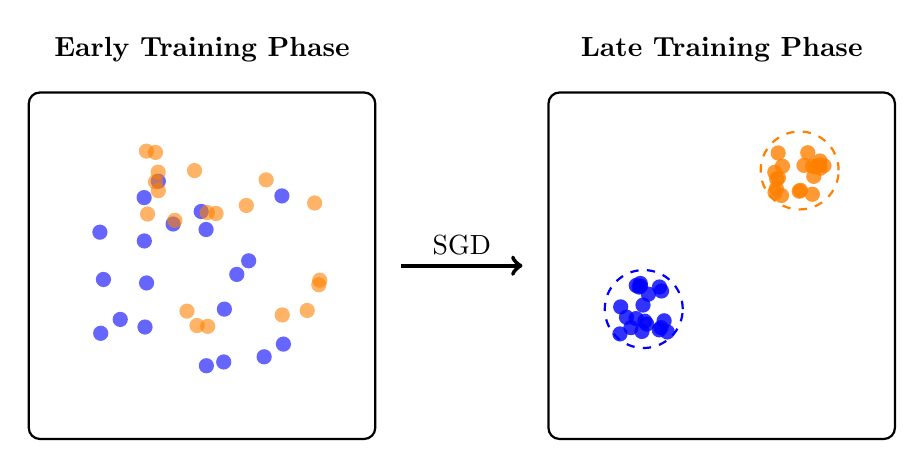
\begin{tikzpicture}[scale=1.1]
    % Initial phase
    \node at (2, 4.5) {\textbf{Early Training Phase}};
    \draw[thick, rounded corners] (0,0) rectangle (4,4);
    
    % Class 1 scattered
    \foreach \i in {1,...,20} {
        \fill[blue, opacity=0.6] (0.8+rnd*2.2, 0.8+rnd*2.2) circle (2.5pt);
    }
    % Class 2 scattered
    \foreach \i in {1,...,20} {
        \fill[orange, opacity=0.6] (1.2+rnd*2.2, 1.2+rnd*2.2) circle (2.5pt);
    }
    
    \draw[->, ultra thick] (4.3, 2) -- (5.7, 2) node[midway, above] {SGD};

    % Late phase
    \node at (8, 4.5) {\textbf{Late Training Phase}};
    \draw[thick, rounded corners] (6,0) rectangle (10,4);
    
    % Class 1 clustered
    \foreach \i in {1,...,20} {
        \fill[blue, opacity=0.8] (6.8+rnd*0.6, 1.2+rnd*0.6) circle (2.5pt);
    }
    % Class 2 clustered
    \foreach \i in {1,...,20} {
        \fill[orange, opacity=0.8] (8.6+rnd*0.6, 2.8+rnd*0.6) circle (2.5pt);
    }
    
    % Ellipses showing volume
    \draw[blue, thick, dashed] (7.1, 1.5) ellipse (0.45 and 0.45);
    \draw[orange, thick, dashed] (8.9, 3.1) ellipse (0.45 and 0.45);

\end{tikzpicture}
\caption{Geometric compression in the representation space $\mathcal{T}$. During the fitting phase, class distributions are heavily entangled with high geometric volume. As training progresses, the network geometrically compresses samples of the same class into tight clusters, reducing $V_k(T)$ while maximizing inter-class margins.}
\label{fig:geometric_compression}
\end{figure}

\begin{horizon}
While the pathology of deterministic mappings invalidates a naive application of the Shannon Information Bottleneck to standard networks, the fundamental intuition remains profoundly compelling. It is conjectured that there exists a generalized ``information-like'' metric that naturally unifies the deterministic and stochastic regimes, capturing the essence of compression without falling prey to infinite singularities. 

Future work might show that replacing Shannon entropy with rigorous topological measures---such as the intrinsic fractal dimension of the data manifold or optimal transport distances between conditional class distributions---yields a generalized IB principle. Such a principle would ideally track generalization cleanly, invariant to whether the network utilizes $\tanh$ or ReLU activations, and without requiring arbitrary binning strategies.

An exciting open question is whether the implicit regularization of stochastic gradient descent inherently minimizes this yet-to-be-defined geometric compression metric. If it is conjectured that the noise in SGD acts as a geometric smoother, driving the representations toward minimal-volume states, this could finally explain the generalization capabilities of heavily overparameterized models through a unified, bottleneck-like mechanism.
\end{horizon}

\section{Summary}
In this chapter, we critiqued the standard Information Bottleneck theory applied to deep learning. We demonstrated that for continuous, deterministic neural networks, the mutual information $I(X; T)$ between the input and hidden layers is technically infinite. Consequently, the widely observed ``compression phase'' in early literature is largely an artifact of two phenomena: the discretization of continuous representations via arbitrary binning, and the shrinking differential entropy caused by saturating activation functions like $\tanh$. 

To salvage the core intuition of the Information Bottleneck, we shifted our perspective from strict Shannon information to geometric clustering. We proved that as the network maps data belonging to the same class into dense regions, the geometric volume and conditional differential entropy of the representations decrease. This geometric viewpoint provides a rigorous framework for understanding how networks abstract away nuisance variables without succumbing to the mathematical pathologies of deterministic mutual information.

\section*{Exercises}
\begin{enumerate}
    \item \textbf{Infinite Information:} Construct a simple 1D continuous random variable $X \sim U(0, 1)$ and a deterministic function $T = 2X$. Calculate $h(T)$. Explain mathematically why $I(X; T) = \infty$ despite the mapping being a simple linear scaling.
    \item \textbf{Saturating Activations:} Let $X \sim \mathcal{N}(0, 1)$ and $T = \sigma(wX)$, where $\sigma(z) = 1/(1+e^{-z})$ is the sigmoid function. Derive an expression for the differential entropy $h(T)$ as a function of the weight $w$. Show analytically that $h(T) \to -\infty$ as $w \to \infty$.
    \item \textbf{ReLU and Binning:} Repeat the empirical binning analysis for a ReLU activation, $T = \max(0, wX)$. Assuming $X \sim \mathcal{N}(0, 1)$, what happens to the binned entropy $H(\hat{T})$ as $w$ increases? Does it show a compression phase similar to saturating activations?
    \item \textbf{Geometric Volume:} Prove that applying an orthogonal weight matrix $W$ (where $W^\top W = I$) to a hidden representation preserves its class-conditional geometric volume $V_k(T)$. 
    \item \textbf{Noise Injection:} Suppose we modify a deterministic network by adding Gaussian noise: $T = f_\theta(X) + \epsilon$, where $\epsilon \sim \mathcal{N}(0, \sigma^2 I)$. Show that $I(X; T)$ is now strictly finite, and express it in terms of $h(T)$ and $\sigma$.
\end{enumerate}

% TODO-CITE: Ensure all named results are cited.
